\chapter{Beschreibung der verschiedenen Messungen und Ergebnisdarstellung}

\section{Verbindungsauf- und abbau}

\begin{figure}[htbp]
\centering
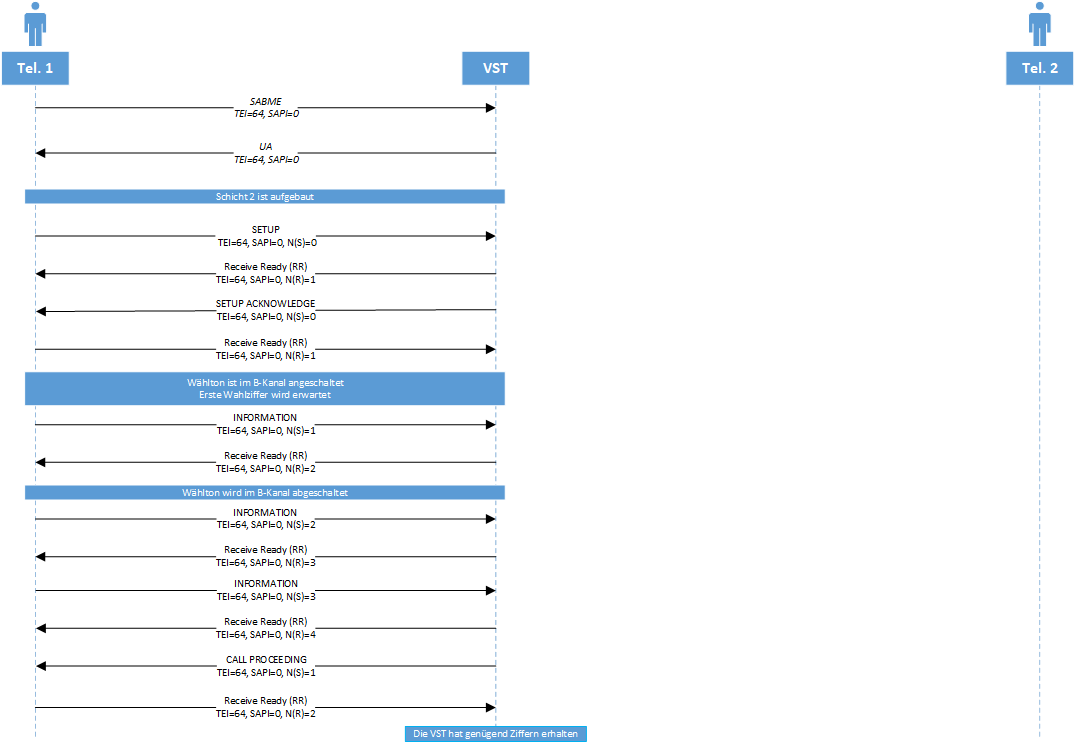
\includegraphics[width=\linewidth]{Graphics/seq1.png}
\caption{Verbindungsauf- und abbau - Teil 1}
\label{fig:seq1}
\end{figure}

\begin{figure}[htbp]
\centering
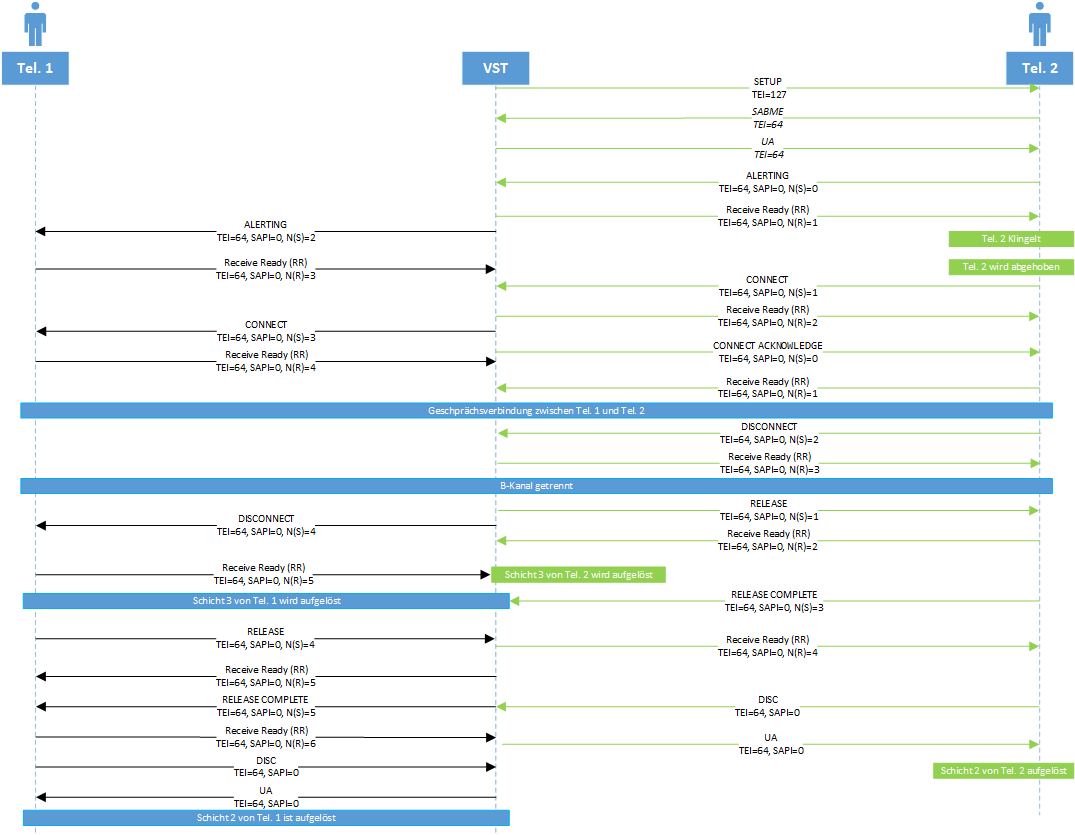
\includegraphics[width=\linewidth]{Graphics/seq2.png}
\caption{Verbindungsauf- und abbau - Teil 2}
\label{fig:seq2}
\end{figure}

\clearpage

Das Sequenzdiagramm zeigt den Ablauf des Verbindungsauf- und abbaus eines
Telefongespr�ches und wurde mit Hilfe des Wireshark-Protokllmitschnitts
erstellt. Aus dem Mitschnitt konnte der Nachrichtenverlauf zwischen Telefon 1
und der \ac{VSt} entnommen werden. Um die Kommunikation zwischen Telefon 2 und
der \acs{VSt} zu visualisieren wurde u.a. ``Die Technik der Netze'' von Gerd
Sigmund, als Quelle genutzt.\\
\newline
Im oberen Abschnitt wird die Schicht-2-Verbindung aufgebaut. Hierzu sendet das
Endger�t eine SABME-Nachricht, welche von der VSt mit einer UA-Nachricht
quittiert wird:\footnote{Die volst�ndigen Frames, denen die Auschnitte
entstammen sind in Anhang B unter der jeweiligen Framenr. zu finden}
\begin{lstlisting}
No.     Time                       Source                Destination           Protocol Info
    338 2018-04-16 17:44:55.129216 User                  Network               LAPD     U P, func=SABME

[...]

No.     Time                       Source                Destination           Protocol Info
    339 2018-04-16 17:44:55.133216 Network               User                  LAPD     U F, func=UA

\end{lstlisting}

Nach dem erfolgreichen Aufbau der Schicht 2 k�nnen nummerierte I-Bl�cke
ausgetauscht werden. Diese sind mit Z�hlern versehen: N(S) z�hlt die gesendeten
Bl�cke, N(R) die empfangenen Bl�cke. Sende- und Empfangsz�hler werden an
dieser Stelle zur�ckgesetzt.\cite{siegmund2002technik}
\newline
Der Aufbau der Schicht 3 beginnt mit der SETUP-Nachricht und findet im
Anschluss statt. Au�erdem lassen sich aus
der SETUP-Nachricht Coding Standard, der angeforderte ISDN-Dienst und die
�bertragungskapazit�t entnehmen:
\newline
\begin{lstlisting}
No.     Time                       Source                Destination           Protocol Info
    340 2018-04-16 17:44:55.163216 User                  Network               Q.931    SETUP
    
[...]

.00. .... = Coding standard: ITU-T standardized coding (0x00)
 ...0 0000 = Information transfer capability: Speech (0x00)
    
[...]

 ...1 0000 = Information transfer rate: 64 kbit/s (0x10)
 
[...]
\end{lstlisting}

Mit Senden von CONNECT ACKNOWLEDGE ist der Aufbau von Schicht 3 abgeschlossen.
Diese Nachricht dient zur Best�tigung, dass der angerufene Teilnehmer die
Verbindung angenommen hat (H�rer abgenommen). Danach wird der B-Kanal im Netz
durchgeschaltet, welcher zuvor zugewiesen wurde.\cite{siegmund2002technik}\\
In diesem Versuch wurde der B-Kanal 1 zugewiesen.

\begin{lstlisting}
No.     Time                       Source                Destination           Protocol Info
    342 2018-04-16 17:44:55.177168 Network               User                  Q.931    SETUP ACKNOWLEDGE

[...]

        .... ..01 = Information channel selection: B1 channel (0x01)
\end{lstlisting}

Im Mitschnitt dieses Versuchs wird die oben genannte CONNECT ACKNOWLEDGE nicht
aufgef�hrt, da aufgrund der Versuchsanordnung nur die Nachrichten
auf Seite von Telefon 1 aufgezeichnet wurden. Es w�re auch m�glich, dass die
CONNECT ACKNOWLEDGE vom Telefon 1 zur \acs{VSt} gesendet wird. Da die Nachricht
aber in diesem Fall keine Beduetung hat, kann diese
entfallen.\cite{siegmund2002technik}
\newline
Nachdem der H�rer von Telefon 2 aufgelegt wurde, wird eine DISCONNECT-Nachricht
gesendet, welche den Abbau der Schicht-3-Verbindung einleitet. Telefon 1
antwortet mit RELEASE. Durch die im Anschluss folgende RELEASE COMPLETE
Nachricht, ausgehend von der \acs{VSt}, ist die Schicht-3-Verbindung abgebaut.
\begin{lstlisting}
No.     Time                       Source                Destination           Protocol Info
    358 2018-04-16 17:45:04.053200 User                  Network               Q.931    RELEASE

No.     Time                       Source                Destination           Protocol Info
    360 2018-04-16 17:45:04.065184 Network               User                  Q.931    RELEASE COMPLETE
\end{lstlisting}

Danach wird Schicht 2 abgebaut, dies geschieht durch eine
DISC-Nachricht, welche mit einer UA quittiert wird.

\begin{lstlisting}
No.     Time                       Source                Destination           Protocol Info
    362 2018-04-16 17:45:11.721200 User                  Network               LAPD     U P, func=DISC
    
No.     Time                       Source                Destination           Protocol Info
    363 2018-04-16 17:45:11.725216 Network               User                  LAPD     U F, func=UA
\end{lstlisting}

\clearpage

\section{Adressierung der Endger�te}\label{tei}
Im Adressfeld des \acs{HDLC}-Protokolls befindet sich der \ac{TEI}. Jedem
Endger�t ist ein solcher Identifier zugeordnet um eine logische Verbindung zwischen
Vermittlungsstelle und Endger�t sicherzustellen. Der TEI kennzeichnet die
Schicht-2-Adresse f�r das ISDN-Ger�t.\cite{brandt2011net}\\
Der TEI kann entweder durch manuelle Einstellung am Ger�t hinterlegt werden
oder von der Vermittlungsstelle zugeteilt werden (TEI-Vergabe). In diesem
Versuch stellt das Endger�t zuerst eine Identity Request, worauf die
Vermittlungsstelle bei Erfolg mit Identity Assigned antwortet. Die Vergabe
erfolgt mittels U-Frame.
\newline
Dem Telefon 1 wird der TEI 64 zugeteilt. Dies ist der erste von der
Vermittlungsstelle zu vergebende Wert. Die Adressen 1-63 k�nnen eingestellt
werden, 64-126 werden von der Vermittlungsstelle zugeteilt. TEI 127 stellt die
Broadcast-Adresse dar.
\newline
\ac{SAPI} bezeichnet ein weiteres Element des HDLC-Adressfeldes und kennzeichnet
den momentan verwendeten ISDN-Schicht-2-Dienst.\cite{brandt2011net}
Bei der TEI-Vergabe ist der Wert des SAPI 63. Dem Protokoll zufolge bedeutet
dies ``Layer 2 management procedures''. Es handelt sich hier um die �bertragung
von paketvermittelten Daten.
\newline


\begin{lstlisting}

No.     Time                       Source                Destination           Protocol Info
     56 2018-04-16 16:30:58.999168 User                  Network               TEI      Identity Request

Frame 56 (8 bytes on wire, 8 bytes captured)
    Arrival Time: Apr 16, 2018 16:30:58.999168000
    [Time delta from previous captured frame: 2.003968000 seconds]
    [Time delta from previous displayed frame: 2.003968000 seconds]
    [Time since reference or first frame: 19639.640168000 seconds]
    Frame Number: 56
    Frame Length: 8 bytes
    Capture Length: 8 bytes
    [Frame is marked: False]
    [Protocols in frame: isdn:lapd:tei_management]
    Point-to-Point Direction: Sent (0)
ISDN
    Channel: D (0)
Link Access Procedure, Channel D (LAPD)
    [Direction: User->Network (0)]
    Address Field: 0xfcff
        1111 11.. .... .... = SAPI: Layer 2 management procedures (63)
        .... ..0. .... .... = C/R: 0
        .... ...0 .... .... = EA1: 0
        .... .... 1111 111. = TEI: 127
        .... .... .... ...1 = EA2: 1
    Control field: U, func=UI (0x03)
        000. 00.. = Command: Unnumbered Information (0x00)
        .... ..11 = Frame type: Unnumbered frame (0x03)
TEI Management Procedure, Channel D (LAPD)
\end{lstlisting}

\clearpage

\begin{lstlisting}
No.     Time                       Source                Destination           Protocol Info
     57 2018-04-16 16:30:59.005200 Network               User                  TEI      Identity Assigned

Frame 57 (8 bytes on wire, 8 bytes captured)
    Arrival Time: Apr 16, 2018 16:30:59.005200000
    [Time delta from previous captured frame: 0.006032000 seconds]
    [Time delta from previous displayed frame: 0.006032000 seconds]
    [Time since reference or first frame: 19639.646200000 seconds]
    Frame Number: 57
    Frame Length: 8 bytes
    Capture Length: 8 bytes
    [Frame is marked: False]
    [Protocols in frame: isdn:lapd:tei_management]
    Point-to-Point Direction: Received (1)
ISDN
    Channel: D (0)
Link Access Procedure, Channel D (LAPD)
    [Direction: Network->User (1)]
    Address Field: 0xfeff
        1111 11.. .... .... = SAPI: Layer 2 management procedures (63)
        .... ..1. .... .... = C/R: 1
        .... ...0 .... .... = EA1: 0
        .... .... 1111 111. = TEI: 127
        .... .... .... ...1 = EA2: 1
    Control field: U, func=UI (0x03)
        000. 00.. = Command: Unnumbered Information (0x00)
        .... ..11 = Frame type: Unnumbered frame (0x03)
TEI Management Procedure, Channel D (LAPD)
\end{lstlisting}

 %ITU T I.241.1
 
\clearpage

\section{W�hlvorgang und Rufnummer�bertragung}%Frage 5, 8, 9, 12
Es gibt zwei M�glichkeiten beim Anruf die Rufnummer \ac{MSN} einzugeben.
Beim Versuch, der in den Abbildungen \label{seq1} und \label{seq2} dargestellt
ist, wurde zun�chst der H�rer von Telefon 1 (100) abgenommen und dann die
Zielrufnummer (200) eingegeben.\\Bei der zweiten Variante wird zuerst die
Rufnummer vollst�ndig eingegeben, bevor der H�rer abgenommen wird.
Dieser W�hlvorgang wird Blockwahl genannt.

\subsection{Einzelwahl}

Bei Einzelwahl werden die Ziffern der Rufnummer in einzelnen
Info-Nachrichten �bertragen:\\

\begin{lstlisting}
No.     Time                       Source                Destination           Protocol Info
    344 2018-04-16 17:44:56.463200 User                  Network               Q.931    INFORMATION
    
[...]    

Called party number: '2'
        Information element: Called party number
        Length: 2
        .... 0001 = Numbering plan: E.164 ISDN/telephony numbering (0x01)
        .000 .... = Number type: Unknown (0x00)
        1... .... = Extension indicator: last octet
        Called party number digits: 2
        E.164 Called party number digits: 2
\end{lstlisting}

\begin{lstlisting}
No.     Time                       Source                Destination           Protocol Info
    346 2018-04-16 17:44:56.895184 User                  Network               Q.931    INFORMATION

[...]

Called party number: '0'
        Information element: Called party number
        Length: 2
        .... 0001 = Numbering plan: E.164 ISDN/telephony numbering (0x01)
        .000 .... = Number type: Unknown (0x00)
        1... .... = Extension indicator: last octet
        Called party number digits: 0
        E.164 Called party number digits: 0
\end{lstlisting}

\clearpage

\begin{lstlisting}
No.     Time                       Source                Destination           Protocol Info
    348 2018-04-16 17:44:57.131184 User                  Network               Q.931    INFORMATION

[...]

Called party number: '0'
        Information element: Called party number
        Length: 2
        .... 0001 = Numbering plan: E.164 ISDN/telephony numbering (0x01)
        .000 .... = Number type: Unknown (0x00)
        1... .... = Extension indicator: last octet
        Called party number digits: 0
        E.164 Called party number digits: 0
\end{lstlisting}

\subsection{Blockwahl}

Bei der Blockwahl ist die \acs{MSN} des Ziels direkt bekannt und wird
in der SETUP-Nachricht �bertragen:
\newline
\begin{lstlisting}
No.     Time                       Source                Destination           Protocol Info
    366 2018-04-16 17:56:17.227216 User                  Network               Q.931    SETUP

[...]

    Calling party number: '100'
        Information element: Calling party number
        Length: 5
        .... 0000 = Numbering plan: Unknown (0x00)
        .000 .... = Number type: Unknown (0x00)
        0... .... = Extension indicator: information continues through the next octet
        .... ..00 = Screening indicator: User-provided, not screened (0x00)
        .00. .... = Presentation indicator: Presentation allowed (0x00)
        1... .... = Extension indicator: last octet
        Calling party number digits: 100
    Called party number: '200'
        Information element: Called party number
        Length: 4
        .... 0001 = Numbering plan: E.164 ISDN/telephony numbering (0x01)
        .000 .... = Number type: Unknown (0x00)
        1... .... = Extension indicator: last octet
        Called party number digits: 200
        E.164 Called party number digits: 200

[...]
\end{lstlisting}

Diesbez�glich unterscheidet sich die SETUP-Nachricht bei den unterschiedlich
W�hlvorg�ngen. Bei Einzelwahl ist die ``Called Party Number'' kein
Element der Nachricht, da die Nummer zu diesem Zeitpunkt nur bei der Blockwahl
bekannt ist.

\section{Nachrichtenelemente}

\begin{figure}[htbp] 
  \centering
     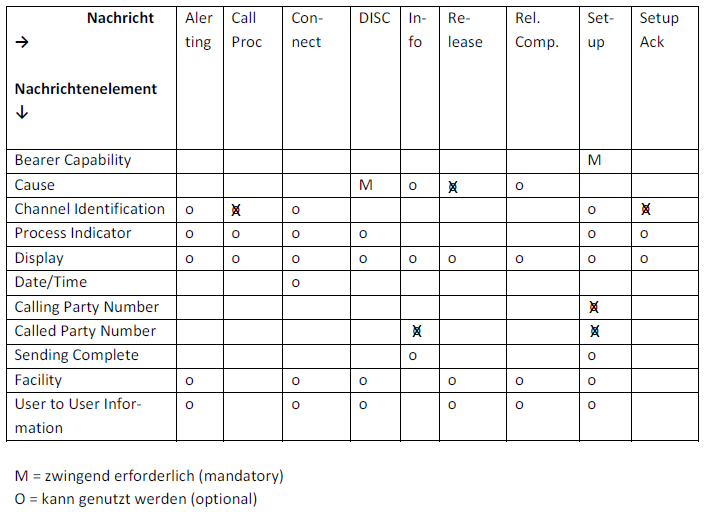
\includegraphics[width=\linewidth]{Graphics/Capture.PNG}
  \caption{Nachrichtenelemente}
  \label{fig:elemente}
\end{figure}

In der Tabelle \label{elemente} ist eine �bersicht gegeben, welche
Nachrichtenelemente in welchen Nachrichten im Protokollmitschnitt des Versuchs
vorkommen (angekreuzt). Die Angaben sind sowohl bei Einzelwahl, als auch bei
Blockwahl identisch, mit einer Ausnahme: ``Called Party Number''.
Dises Element ist lediglich bei der Blockwahl in der SETUP-Nachricht zu finden.
Bei Einzelwahl ist die MSN zu der geroutet werden soll zum Zeitpunkt der
SETUP-Nachricht nicht bekannt.

\clearpage

\section{SETUP-Nachricht}
Die folgende Tabelle wurde anhand des Mitschnitts, genauer mit dem Rahmen der
SETUP-Nachricht bei Blockwahl, erstelltt. Gleichzeitig wurden Informationen aus
dem Standard herangezogen, um die Ergebnisse zu
vergleichen.\cite{recommendation1998digital}

\begin{figure}[htbp] 
     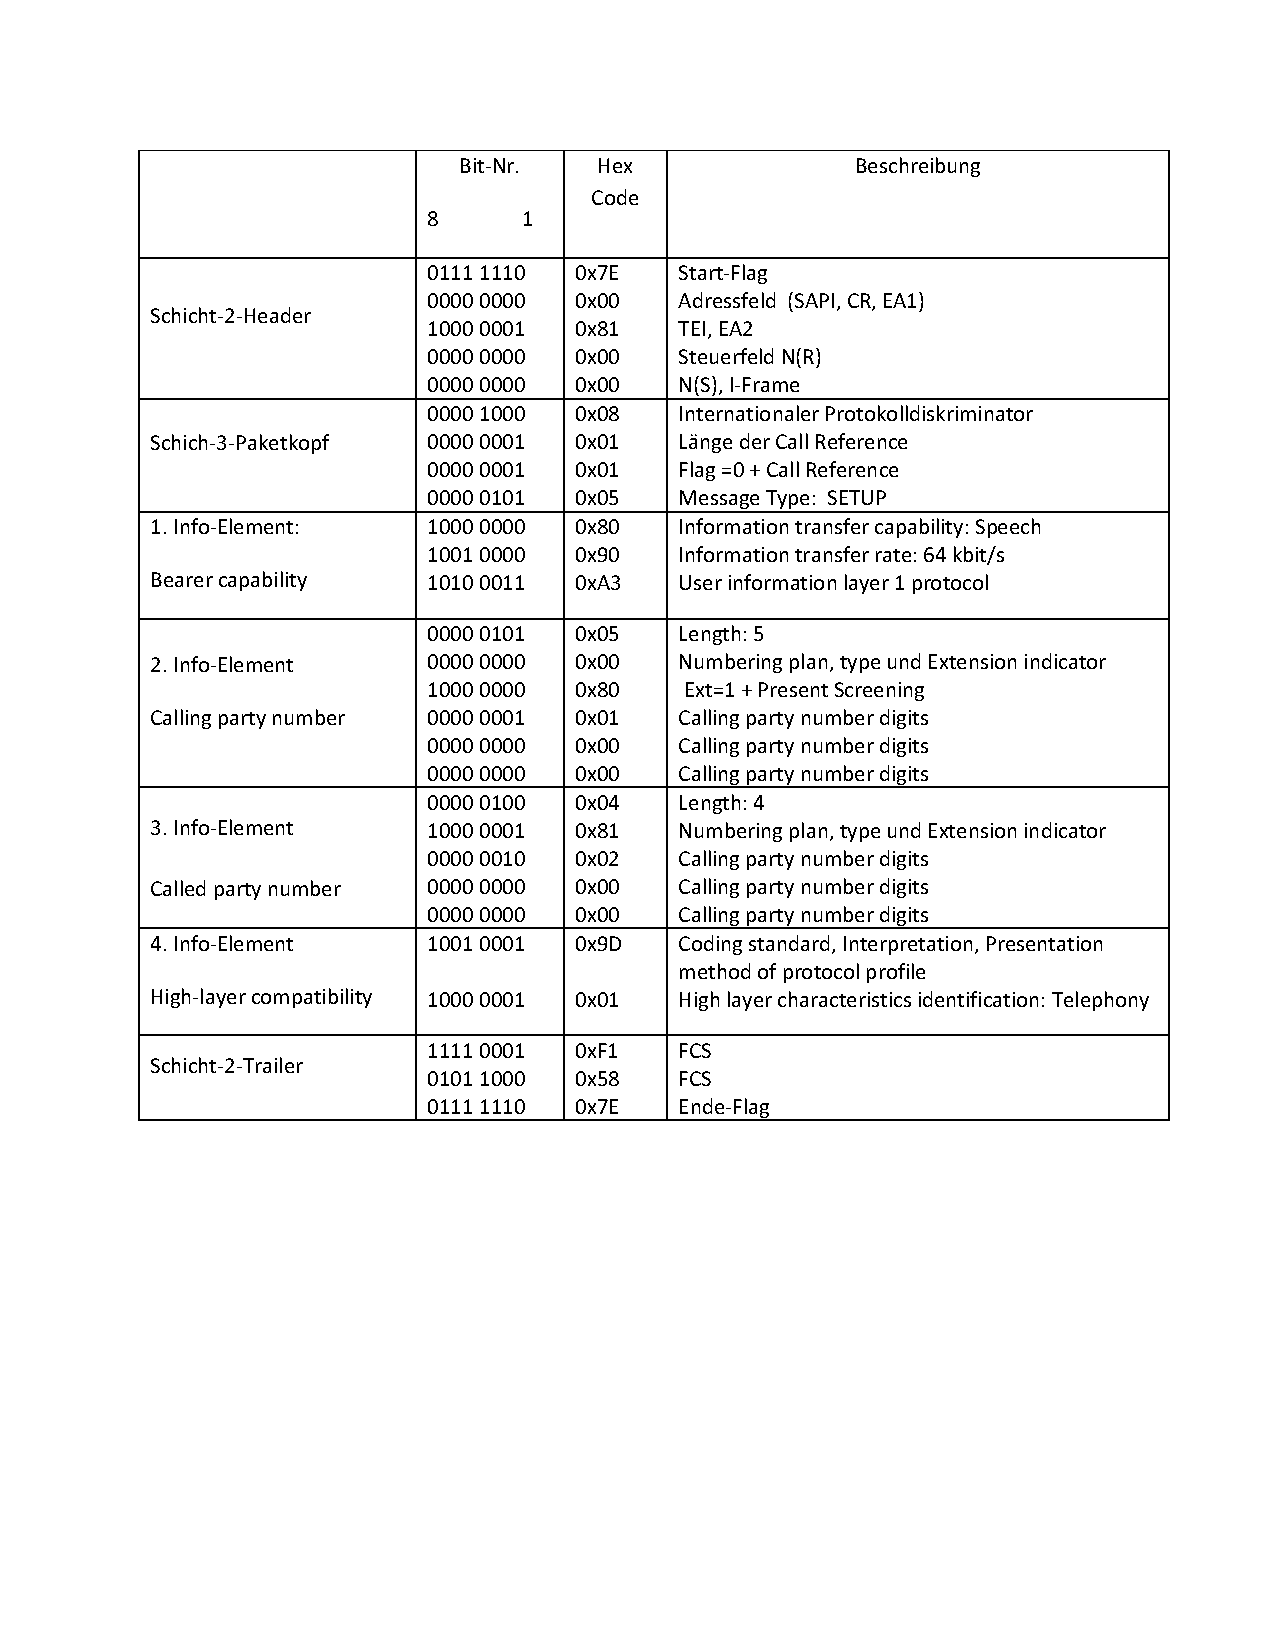
\includegraphics[width=\linewidth]{Graphics/Bit.pdf}
  \caption{SETUP-Nachricht in Schicht-2-Rahmen eingebunden}
  \label{fig:setup}
\end{figure}
